\documentclass[a4paper, 12pt, final, garamond]{book}
\usepackage{cours-preambule}

\raggedbottom

\makeatletter
\renewcommand{\@chapapp}{\'Electrocin\'etique -- chapitre}
\makeatother

\begin{document}
\setcounter{chapter}{4}

\chapter{TD~: circuits \'electriques en RSF}

\section{Impédance équivalente}
Déterminer l’impédance complexe équivalente de chacun des dipôles ci-dessous en RSF.
\begin{center}
    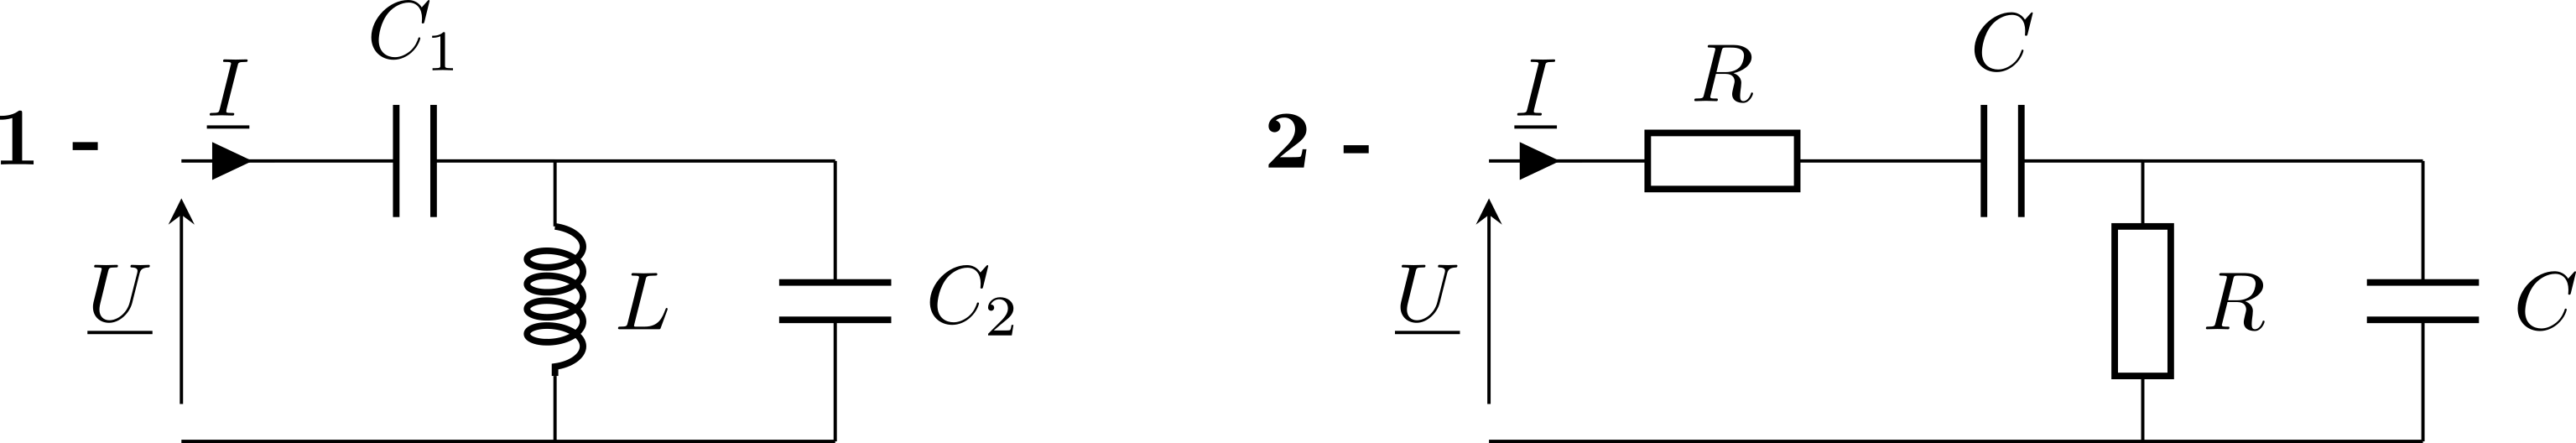
\includegraphics[width=.8\linewidth]{exo1_plain}
\end{center}

\section{Circuit RL série en RSF}
On considère le circuit ci-contre en régime sinusoïdal forcé, où la source de
tension impose $e(t) = E\cos(\wt)$ avec $E > 0$.

\begin{minipage}{0.60\linewidth}
    \begin{enumerate}
        \item Déterminer l'amplitude de $u$ à «~très haute~» ($\w\rightarrow\infty$)
            et «~très basse~» ($\w\rightarrow0$) fréquence.
        \item Exprimer l'amplitude complexe $\ul{U}$ de $u(t)$ en fonction de $E$,
            $R$, $L$ et $\w$.
        \item Les tensions $e$ et $u$ peuvent-elles être en phase~? En opposition de
            phase~? En quadrature de phase~? Préciser le cas échéant pour quelle(s)
            pulsation(s).
    \end{enumerate}
\end{minipage}
\hfill
\begin{minipage}{0.35\linewidth}
    \begin{center}
        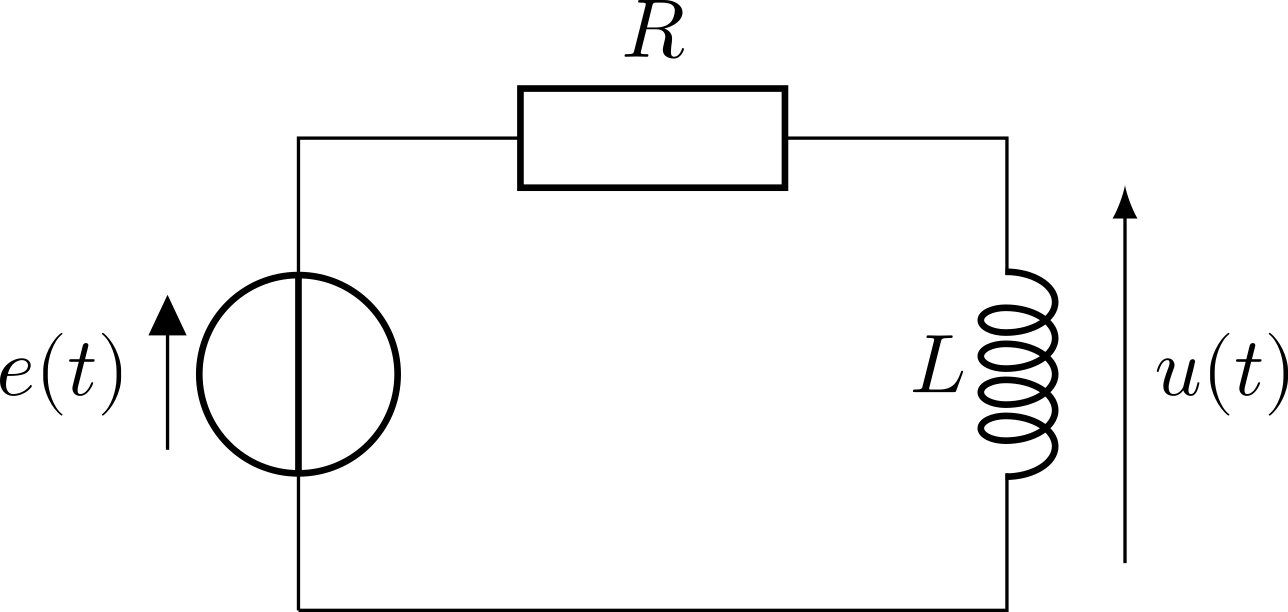
\includegraphics[width=\linewidth]{exo2_plain}
    \end{center}
\end{minipage}

\section{Exploitation d'un oscillogramme en RSF}
On considère le circuit ci-dessous. On pose $e(t) = E_m\cos(\wt)$ et $u(t) =
U_m\cos(\wt+\f)$. La figure ci-dessous représente un oscillogramme réalisé à la
fréquence $f = \SI{1.2e3}{Hz}$, avec $R = \SI{1.0}{k\Omega}$ et $C =
\SI{0.10}{\micro F}$.
\begin{center}
    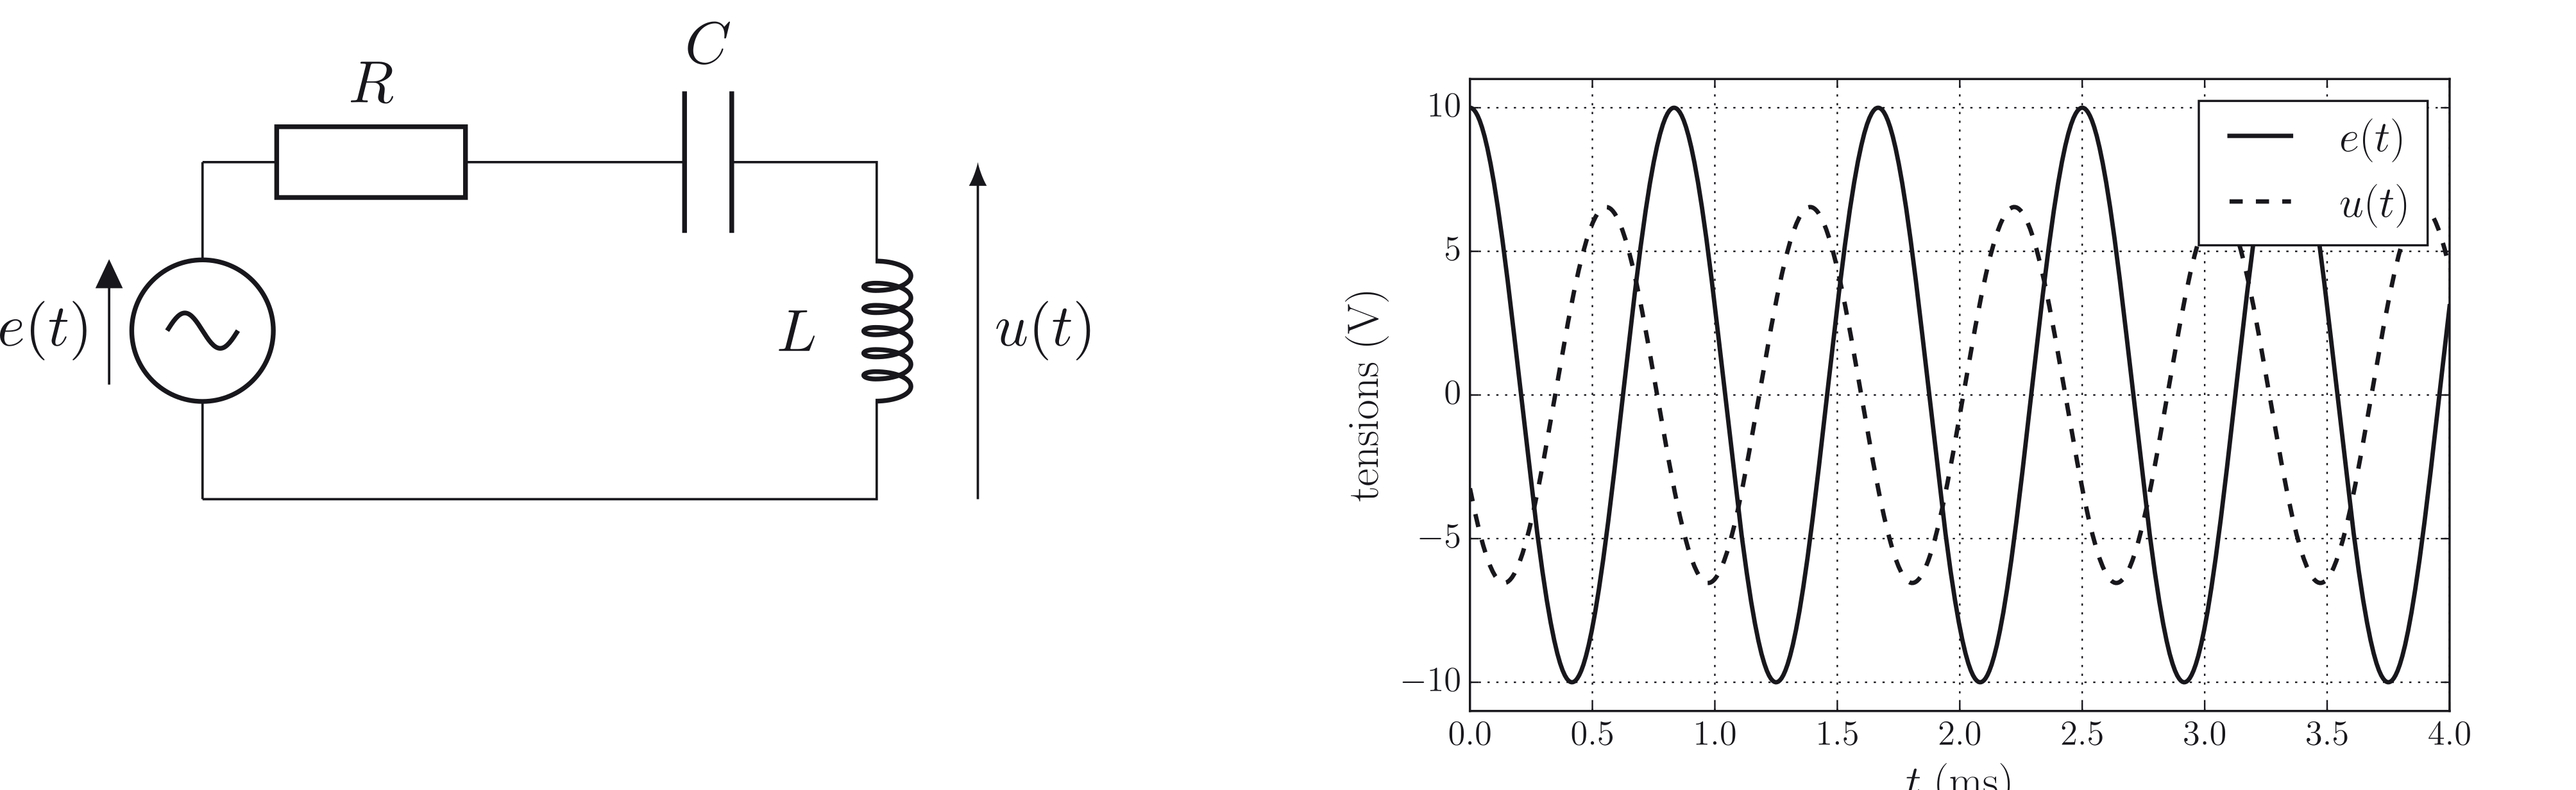
\includegraphics[width=\linewidth]{exo3_plain}
\end{center}
\begin{enumerate}
    \item Déduire de cet oscillogramme les valeurs expérimentales de $E_m$,
        $U_m$ et $\f$.
    \item Exprimer $U_m$ et $\f$ en fonction des composants du circuit.
    \item En déduire la valeur numérique de l'inductance $L$ de la bobine.
\end{enumerate}

\section{Comportement d'un circuit à haute et basse fréquence}
On considère le circuit ci-contre. On pose $e(t) = E_m\cos(\wt)$ et $u(t) =
U_m\cos(\wt+\f)$.

\begin{minipage}{0.60\linewidth}
    \begin{enumerate}
        \item Définir les signaux complexes $\ul{e}(t)$ et $\ul{u}(t)$ puis les
            amplitudes complexes $\ul{E}$ et $\ul{U}$ associées aux tensions
            $e(t)$ et $u(t)$, respectivement.
        \item Établir l'expression de $\ul{U}$ en fonction de $E_m$, $R$, $L$,
            $C$ et $\w$.
        \item En déduire les expressions de $U_m$ et de $\f$ en fonction de
            $E_m$, $R$, $L$, $C$ et $\w$.
        \item Déterminer les valeurs limites de $U_m$ à très basse et très haute
            fréquence. Ces résultats étaient-ils prévisibles par une analyse
            qualitative du montage~?
    \end{enumerate}
\end{minipage}
\hfill
\begin{minipage}{0.35\linewidth}
    \begin{center}
        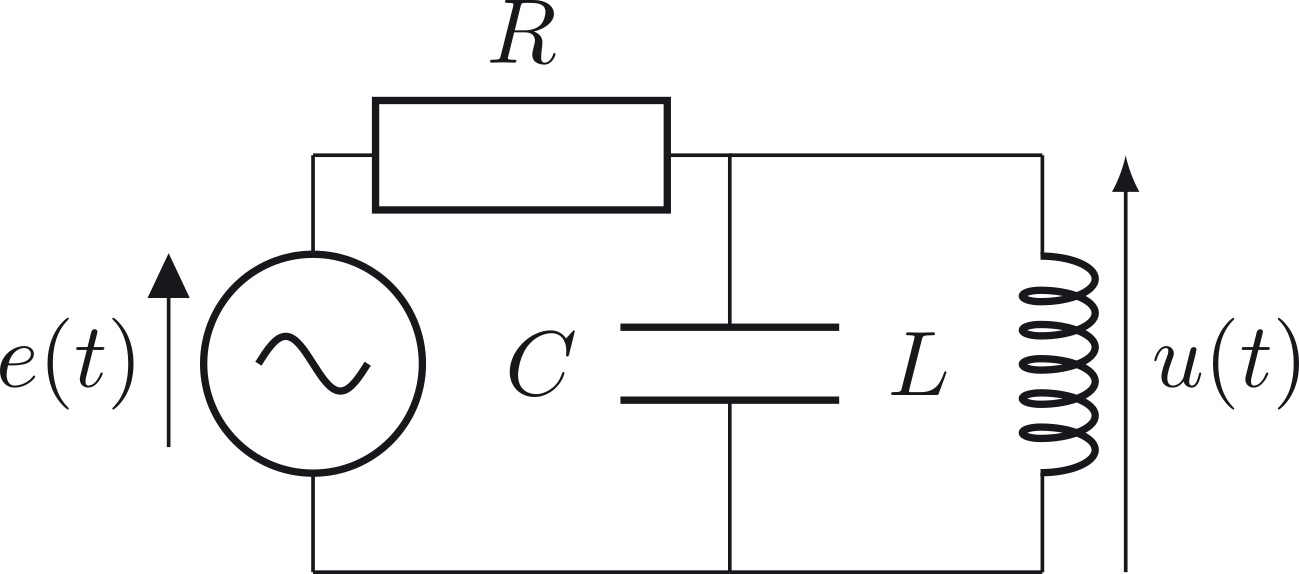
\includegraphics[width=\linewidth]{exo4_plain}
    \end{center}
\end{minipage}

\section{Dipôle inconnu}

\begin{minipage}{0.60\linewidth}
    Dans le montage ci-contre, le GBF délivre une tension $e(t)$ sinusoïdale de
    pulsation $\w$, $R$ est une résistance et $D$ un dipôle inconnu. On note
    $u(t) = U_m\cos(\wt)$ et $v(t) = V_m\cos(\wt+\F)$ les tensions aux bornes
    respectivement de $R$ et $D$. On visualise à l'oscilloscope $v(t)$ et
    $u(t)$, et on obtient le graphe ci-dessous.
\end{minipage}
\begin{minipage}{0.35\linewidth}
    \begin{center}
        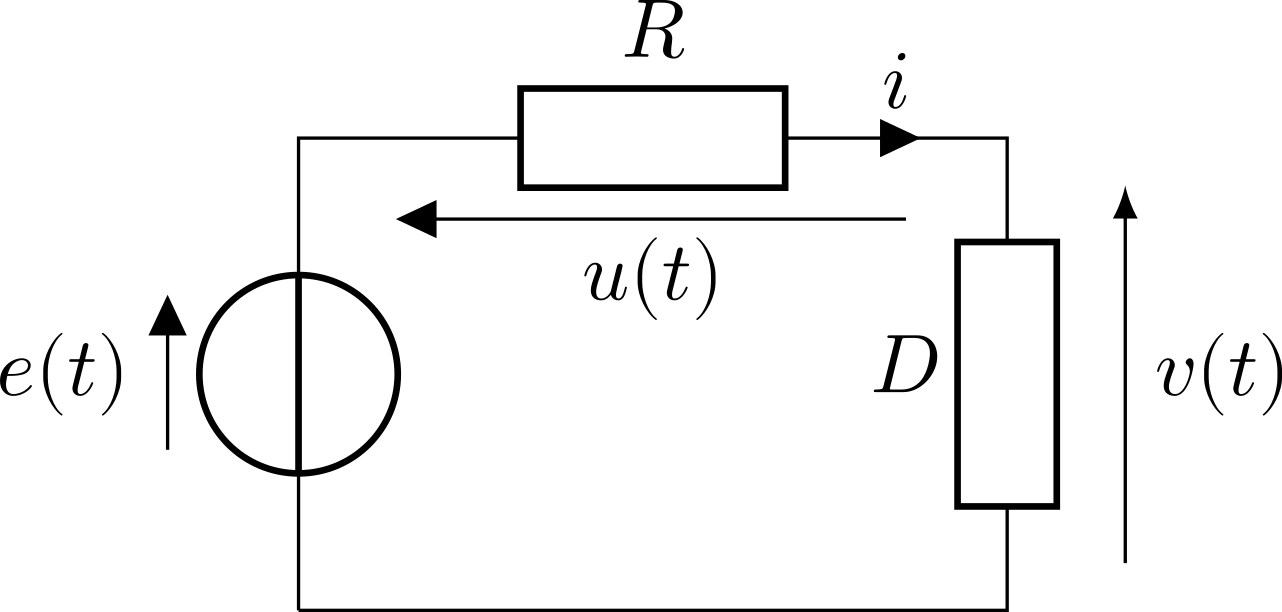
\includegraphics[width=\linewidth]{exo5_plain}
    \end{center}
\end{minipage}

\begin{center}
    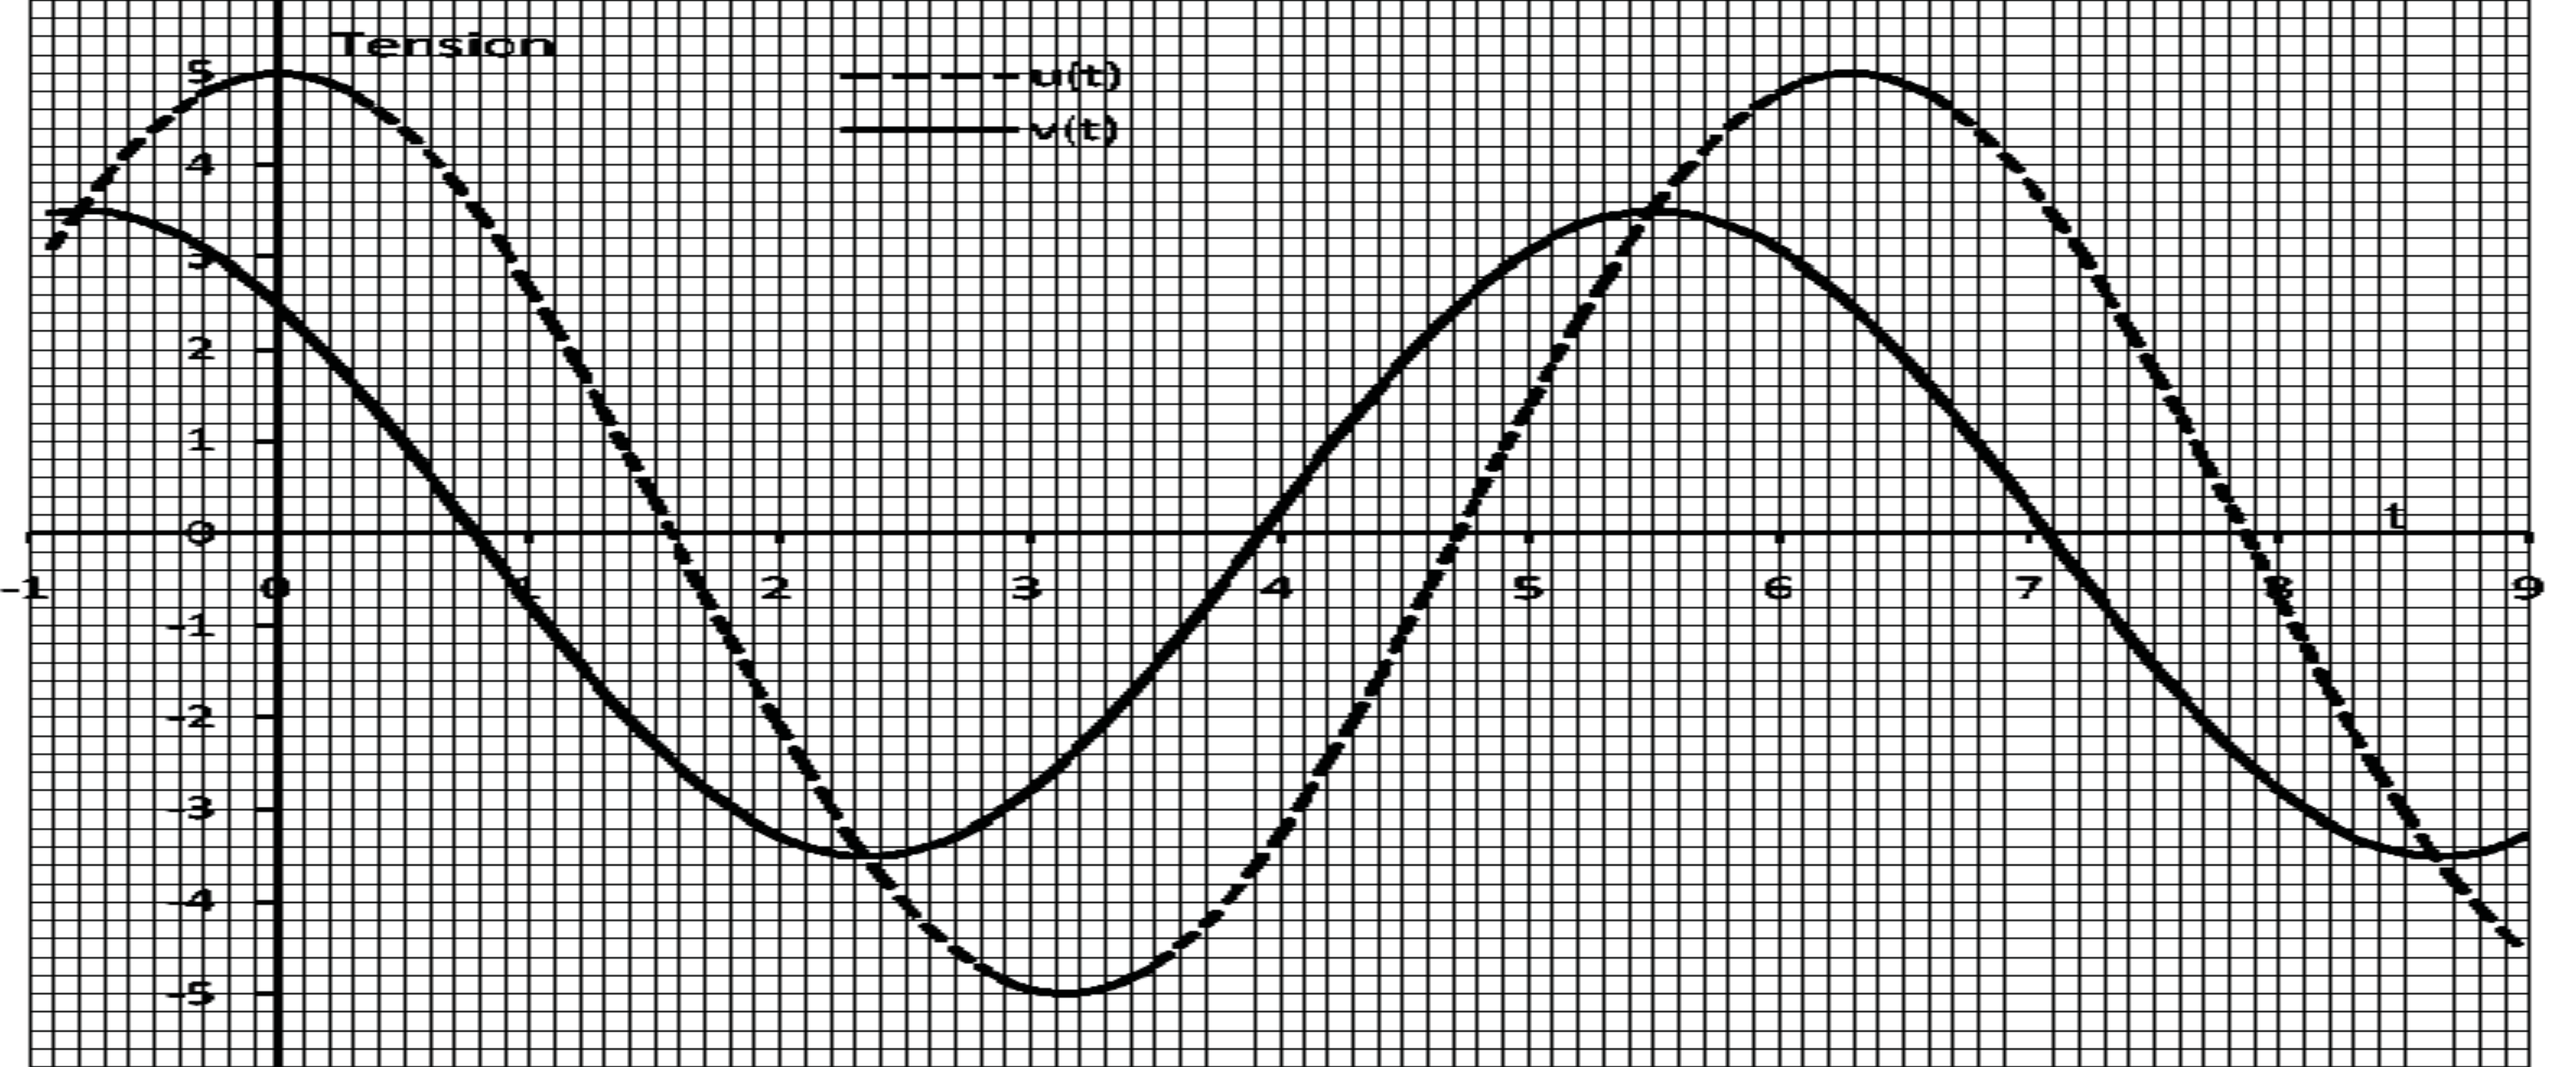
\includegraphics[width=\linewidth]{exo5_plain-2}
\end{center}

L'unité de l'axe des temps est $\SI{e-2}{s}$, et celle de l'axe des tensions est
\SI{1}{V}. On utilise ces résultats graphiques pour déterminer les
caractéristiques de $D$, sachant que $R = \SI{100}{\Omega}$.

\begin{enumerate}
    \item Déterminer $V_m$, $U_m$ ainsi que la pulsation $\w$ des signaux
        utilisés.
    \item La tension $v$ est-elle en avance ou en retard sur la tension $u$~? En
        déduire le signe de $\F$. Déterminer la valeur de $\F$ à partir du
        graphe.
    \item On note $\ul{Z} = X + \jj Y$ l'impédance complexe du dipôle $D$.
        \begin{enumerate}
            \item Déterminer les valeurs de $X$ et $Y$ à partir des résultats
                précédents.
            \item Par quel dipôle (condensateur, bobine, résistance) peut-on
                modéliser $D$~?
        \end{enumerate}
\end{enumerate}

\section{Obtention d'une équation différentielle}
\begin{minipage}{0.60\linewidth}
    En utilisant les complexes, montrer que la tension $u(t)$ est solution de
    l'équation différentielle
    \[4\tau^2 \dv[2]{u}{t} + R\tau \dv{u}{t} + u(t) = e(t)
        \qavec
        \tau = RC
    \]
\end{minipage}
\hfill
\begin{minipage}{0.35\linewidth}
    \begin{center}
        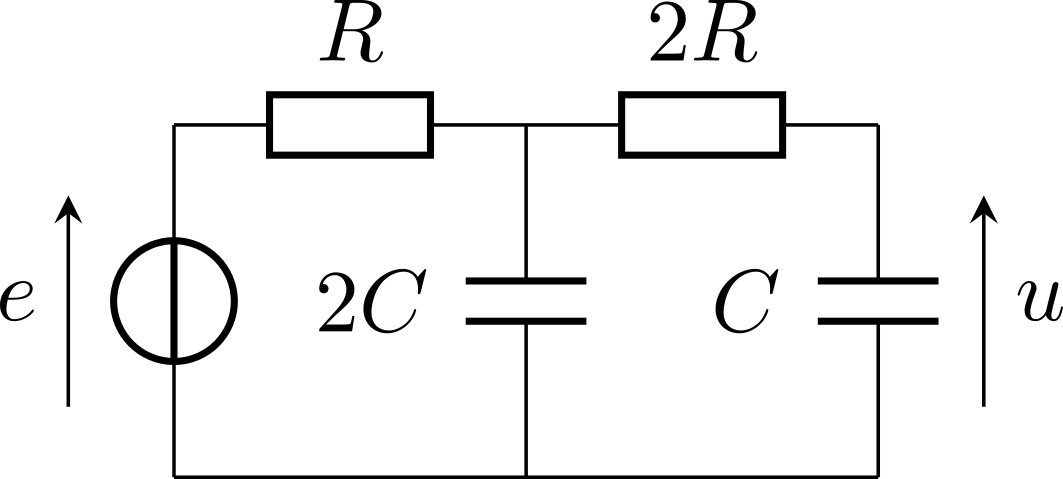
\includegraphics[width=\linewidth]{exo6_plain}
    \end{center}
\end{minipage}

\section{Déphasage, pulsation et impédance}
\begin{minipage}{0.55\linewidth}
    On considère le circuit en RSF. Déterminer l'expression de la pulsation $w$
    de la tension sinusoïdale $e(t) = E\cos(\wt)$ pour que le courant $i(t)$
    soit en phase avec $e(t)$. \bigbreak
    \textit{Indication}~: utiliser l'impédance équivalente constituée de $C$,
    $L$ et $R_2$.
\end{minipage}
\hfill
\begin{minipage}{0.40\linewidth}
    \begin{center}
        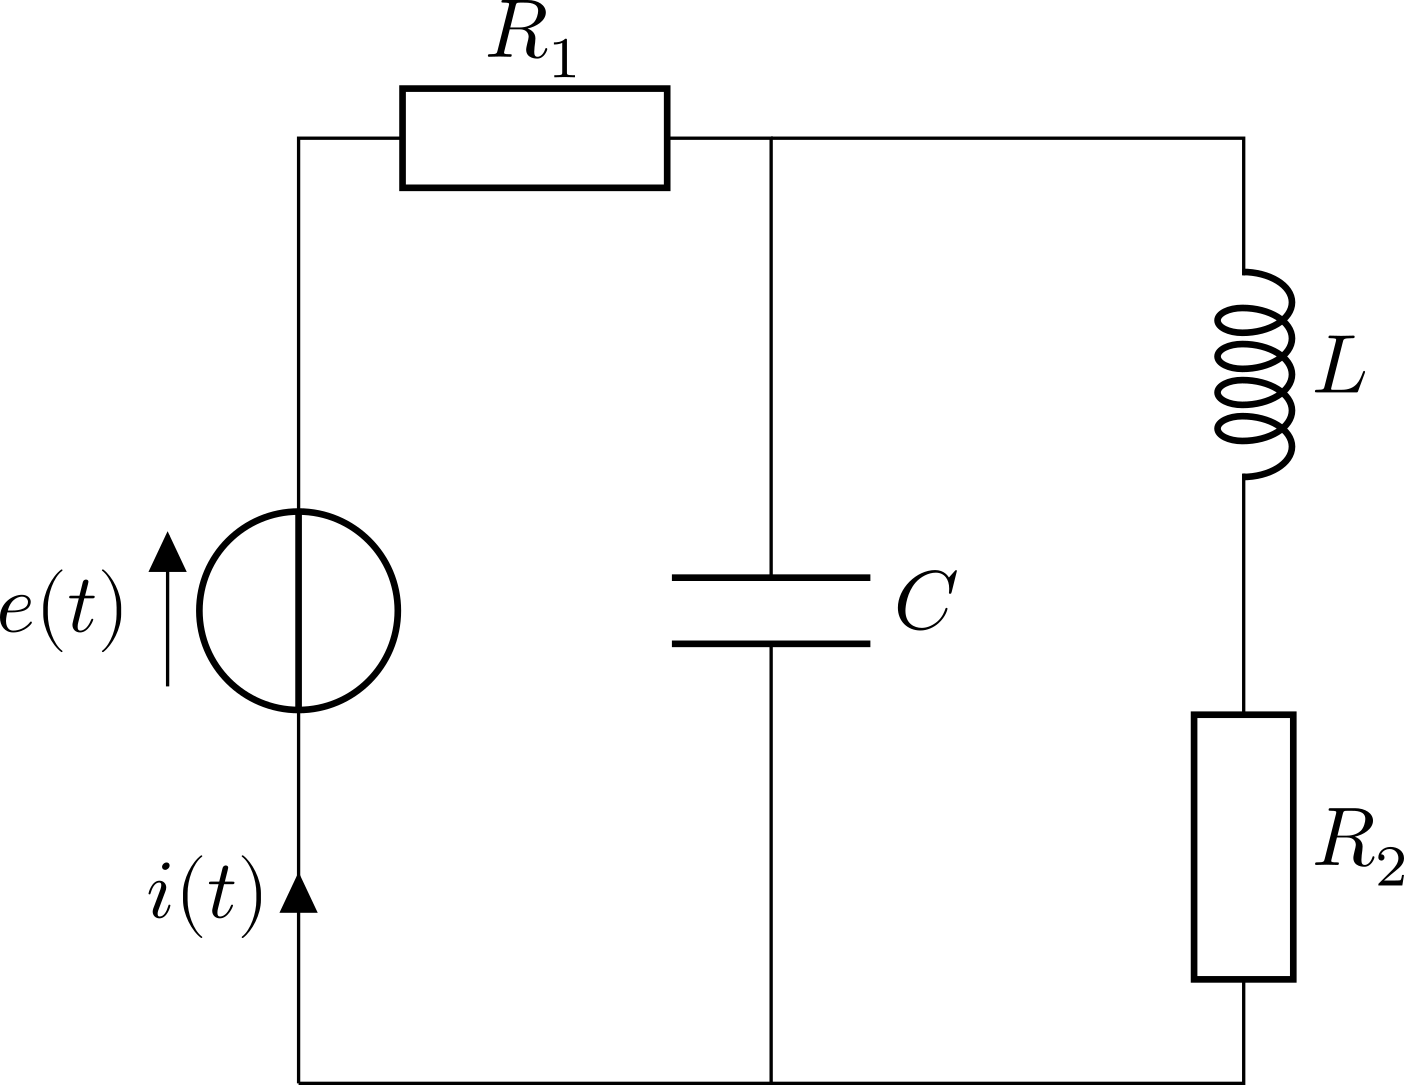
\includegraphics[width=\linewidth]{exo7_plain}
    \end{center}
\end{minipage}

\section{Oscillateur à quartz}
\begin{minipage}{0.60\linewidth}
    Un quartz piézo-électrique se modélise par un condensateur (de capacité
    $C_0$) placé en parallèle avec un condensateur (de capacité $C$) en série
    avec une inductance $L$. On se place en régime sinusoïdal forcé de pulsation
    $\w$.
\end{minipage}
\hfill
\begin{minipage}{0.35\linewidth}
    \begin{center}
        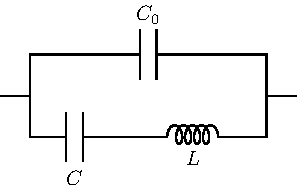
\includegraphics[width=\linewidth]{quartz_plain}
    \end{center}
\end{minipage}

\begin{enumerate}
    \item Donner l'impédance équivalente $\ul{Z}$ de l'oscillateur.
    \item Trouver la pulsation pour laquelle l'impédance de l'ensemble est
        nulle, puis celle pour laquelle elle est infinie.
    \item Tracer l'allure de $|\ul{Z}(\w)|$.
    \item Comment la courbe précédente serait-elle modifiée si on prenant en
        compte les résistances de chacun des composants~?
\end{enumerate}

\end{document}
